\section{Characterizing weakly-coupled carbon spins}
Using the knowledge of the interaction between the NV-center and individual nuclear spins it is possible to implement basic gates and characterize the spins.
This section will first explain how basic gates can be implemented on weakly coupled carbon spins.
These gates are then used to measure the precession frequency and $T_2&*$ for individual carbon spins.

\subsection{Basic operations}
In order to implement basic gates on a nuclear spin we make use of the conditional rotation that occurs on the resonance given by \cref{eq:res_dip_loc}.
At the resonant condition the nuclear spin rotates about one of two anti-parallel axes depending on the electronic-spin state.
The angle of the rotation is proportional to the number of pulses on the electron ($N$).
By sweeping the number of pulses to perform a $\pi/2$ rotation a maximally entangling gate is performed.
We define the axis of rotation of this operation as the $x$-axis and call the operation the $\pm \mathrm{x}$-gate.

By bringing the electron in a superposition, sweeping the number of pulses on the electron and measuring the contrast an oscillation can be measured.
This oscillation can be used to calibrate the $\pm \mathrm{x}$-gate.
For twice the number of pulses ($N_{\pm\mathrm{x}}$) required to implement the $\pm \mathrm{x}$-gate the contrast is -1 for an ideal $\pm \mathrm{x}$-gate.
The fidelity with which the oscillation can be sweeped to -1 is equal to the squared fidelity with which the $\pm \mathrm{x}$-gate can be implemented.

The $\pm\mathrm{x}$-gate forms the basis of our control over weakly coupled spins.
\Cref{fig:gate_circuit_pm-x} shows how the $\pm \mathrm{x}$-gate is depicted in a circuit-diagram.
A non entangling rotation can be implemented by placing the electron in an eigenstate before performing the $\pm\mathrm{x}$-operation.
% Van der Sar et al. \citep{Sar2012DecoherenceProtected} have demonstrated how to integrate regular operations on the NV-spin with a decoupling sequence.
By letting the phase of the carbon evolve we are able to apply operations on the carbon-spin with arbitrary phase.


\begin{figure}[htbp]
    \centering
        \mbox{
        \Qcircuit @C=1em @R=.7em {
         \lstick{\ket{\Psi}_e} &\ctrl{1}  &\qw\\
          \lstick{\ket{\Psi}_\mathrm{C}} &\gate{\pm \mathrm{x} }  &\qw}}
    \caption{The $\pm\mathrm{x}$-gate performs an x-rotation on the carbon ($\ket{\Psi}_\mathrm{C}$) when the electron is in the $\ket{0}_e$-state. It performs a $-\mathrm{x}$-rotation when the electron is in the $\ket{1}_e$-state.}
    \label{fig:gate_circuit_pm-x}
\end{figure}

The $\pm\mathrm{x}$-gate has been calibrated for several spins.
The parameters used to implement $\pm\mathrm{x}$-gates are listed in \cref{tbl:gate_parameters}.
Of these carbon-1 and carbon-4 were selected for the experiments.

\begin{table}[htbp]
    \centering
    \caption{Parameters used to implement $\pm\mathrm{x}$-gates.}
    \begin{tabular}{cccc}
    Carbon &  $ N $ &  $\tau$ & total gate time\\ \hline
    1 &  18 & { }9.420 $\mu$s & 339 $\mu$s \\
    2 & 26 & { }6.620 $\mu$s & 344 $\mu$s \\
    3 & 14 & 18.564 $\mu$s & 520 $\mu$s \\
    4 &  40 & { }6.456 $\mu$s & 516 $\mu$s
    \end{tabular}
    \label{tbl:gate_parameters}
\end{table}



\subsection{Carbon Ramsey experiment }
By performing a Ramsey experiment the precession and dephasing-time $T_2^*$ can be determined.
The precession frequencies are required to calculated the phase required to implement operations with the correct phase.
By measuring the precession frequency it is also possible to test our estimation for the hyperfine parameters.

In an ordinary Ramsey experiment a qubit is brought to the equator of the Bloch-sphere where it precesses for a time $\tau $ before it is read out along the x-direction.
A carbon-Ramsey experiment is similar.
\begin{figure}[htbp]
        \centering
        \mbox{
        \Qcircuit @C=1em @R=.7em {
        \lstick{\ket{0}}          & \gate{\mathrm{y}}  & \ctrl{1}    & \dashedGate{\mathrm{x}}  & \multigate{1}{T}  & \dashedGate{\mathrm{-x}}      &\ctrl{1}          & \gate{\mathrm{-y}}  &  \meter \\
        \lstick{\rho_\mathrm{m}}         & \qw              &  \gate{\pm \mathrm{x}}    &  \qw& \ghost{T}        & \qw & \gate{\pm \mathrm{x}}      & \qw       &\qw&}}
    \caption{Gate circuit depicting an uninitialized carbon Ramsey. $T$ is the free evolution time. $\mathrm{x}$ and $\mathrm{y}$ are $\pi/2$ pulses along the $x$ and $y$ axis respectively. The dotted gates are not present when the electron is protected against decoherence by dynamical decoupling during the free evolution time $T$.}
    \label{fig:gate_circuit_nuclear_ramsey}
\end{figure}

The gate circuit of the uninitialized carbon-Ramsey experiment is depicted in \cref{fig:gate_circuit_nuclear_ramsey}.
The first pulse brings the electronic spin in the $\ket{X}$-state.
Because the carbon starts out in a mixed state the two-qubit system can be described by the tensor product of two density matrices:
\begin{equation}
    \rho_X \otimes \rho_m = \rho_X \otimes \rho_{X} +\rho_X \otimes \rho_{-X}
\end{equation}
By applying the $\pm{\mathrm{x}}$-gate  the electronic-spin picks up a phase depending on the nuclear spin-state:
\begin{equation}
     \rho_Y \otimes \rho_{X} +\rho_{-Y} \otimes \rho_{-X}
    \label{eq:density_after_Ren}
\end{equation}
In this state it is either left to freely evolve for a time $T$ while the electronic spin is protected against decoherence trough dynamical decoupling, or a $\pi/2$-pulse is applied to bring the electron back to the poles of the Bloch-sphere.
If the extra $\pi/2$-pulse is applied the system is in the following state before the free evolution.
\begin{equation}
     \rho_0 \otimes \rho_{X} +\rho_{1} \otimes \rho_{-X}
\end{equation}
Because the electronic spin is in a different state for $\rho_{X}$ and $\rho_{-X}$ they evolve with different frequencies.
After the free evolution another $\pi/2$-pulse is applied to bring the electronic spin back into the $xy$-plane.

The final part of the circuit reads out the nuclear spin along the $x$-direction for $\ket{Y}_e$ and along the $-x$-direction for $\ket{-Y}_e$.
The phase picked up during free evolution shows up as an oscillation between $\ket{0}_e$ and $\ket{1}_e$ in the readout.

\subsubsection{Determining the precession frequency}
Because the uninitialized carbon-Ramsey evolves with two frequencies we expect the measured oscillation to be the sum of two cosines as described by \cref{eq:carbon_ramsey_expected}:
\begin{equation}
    c_1 - c_2 \cos(\omega_L \tau ) -c_3  \cos (\tilde{\omega} \tau )
    \label{eq:carbon_ramsey_expected}
\end{equation}
Where $ \tilde\omega =   \sqrt{(\omega_L+A_\parallel) ^2 + A_\perp^2} $ and $c_1$, $c_2$ and $c_3$ are constants.


\begin{figure}[htbp]
    \begin{subfigure}[t]{0.49\textwidth}\centering
        \caption{}
        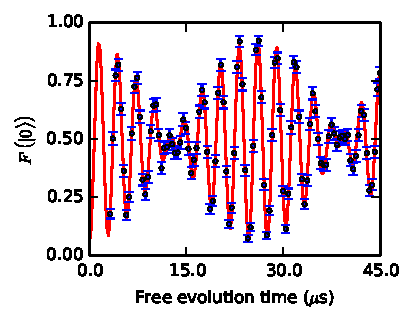
\includegraphics{Img/CarbonRamsey_C1.pdf}
        \label{fig:CR_C1}
    \end{subfigure}
    \begin{subfigure}[t]{0.49\textwidth}\centering
        \caption{}
        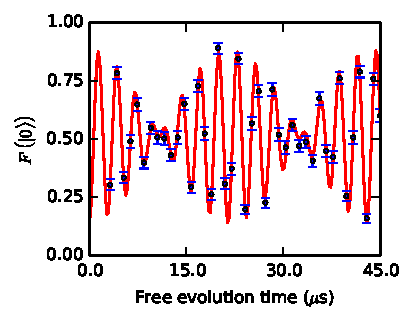
\includegraphics{Img/CarbonRamsey_C4.pdf}
        \label{fig:CR_C4}
    \end{subfigure}
    \caption{The uninitialized carbon-Ramsey experiment shows an oscillation due to the phase picked up during free evolution.
    \subref{fig:CR_C1} shows data for carbon-1 and \subref{fig:CR_C4} for carbon-4.
    The measured frequencies were, for carbon-1: $\omega_{L,C1} = 2\pi\cdot 325.81 \pm 0.25$ and  $\tilde \omega_{\mathrm{C1}}= 2\pi\cdot 364.41 \pm 0.23$, and for carbon-4: $\omega_{L,C4} =  2\pi\cdot 325.94 \pm 0.40$ and $\tilde \omega_{\mathrm{C4}} = 2\pi\cdot 371.52 \pm 0.39 $.}
    \label{fig:Uninitialized_carbon_ramsey}
\end{figure}

\Cref{fig:Uninitialized_carbon_ramsey} shows the results for an uninitialized carbon-Ramsey experiment.
The data was fitted to a sum of two cosines in order to determine the frequencies.

The Larmor frequencies measured are $\omega_{L,C1} = 2\pi\cdot 325.81 \pm 0.25\, \mathrm{kHz}$  for carbon-1 and  $\omega_{L,C4} =  2\pi\cdot 325.94 \pm 0.40\, \mathrm{kHz}$for carbon-4.
Both the measured Larmor frequencies agree with the magnetic field of $304\, \mathrm{G}$ within two standard deviations.

Based on the estimated hyperfine parameters we expect $\tilde\omega_{\mathrm{C1}} \approx 2\pi\cdot 364.7\, \mathrm{kHz}$for carbon-1 and $\tilde \omega_{\mathrm{C4}} \approx 2\pi\cdot 371.4\, \mathrm{kHz}$ for carbon-4.
For carbon-1 $\tilde \omega_{\mathrm{C1}}= 2\pi\cdot 364.41 \pm 0.23\, \mathrm{kHz}$ was measured
and for carbon-4 $\tilde \omega_{\mathrm{C4}} = 2\pi\cdot 371.52 \pm 0.39 \, \mathrm{kHz}$ was measured.
Both these values are in good agreement with experiment, an indication that our hyperfine estimation is accurate.


\subsubsection{Measuring $T_{2,\mathrm{C}}^* $}
% Lange carbon ramseys van Hans sil01 140506 #53 en 56 +T2* analyse.
% hoeveel pulses voor de lange tau? belangrijk voor T2*
To determine $T_{2,\mathrm{C}}^* $ for normal operation an uninitialized carbon-Ramsey was performed where the electron was dynamically decoupled during the free evolution time.
Dynamical decoupling was performed at $\tau = 8\cdot \tau_L$ by varying the number of pulses $N$. $\tau_L$ is the Larmor period $1/\omega_L$ of the carbon.
Because the electron is constantly flipped the carbon will precess with an average frequency of $\omega_{\mathrm{DD}} = (\omega_L +\tilde{\omega} )/2$.
By undersampling with a frequency slightly detuned from the precession frequency ($\omega_{\mathrm{DD}}$) a decaying cosine can be observed where the 1/e time of the envelope is equal to $T_2^*$.
Because this decaying cosine can be measured for a relatively long time ($\sim \mathrm{ms}$) this method can also be used to accurately determine the precession frequency.

\begin{figure}[htbp]
    \begin{subfigure}[t]{0.49\textwidth}\centering
        \caption{}
        \includegraphics{Img/Carbon1_T2star.pdf}
        \label{fig:T2star_carbon1}
    \end{subfigure}
    \begin{subfigure}[t]{0.49\textwidth}\centering
        \caption{}
        \includegraphics{Img/Carbon4_T2star.pdf}
        \label{fig:T2star_carbon4}
    \end{subfigure}
    \caption{Carbon-Ramsey experiment to determine $T_2^*$ for nuclei while decoupling the electron.
    Dynamical decoupling during evolution is implemented at $8\cdot \tau_L$ of the carbon spin. Free evolution time is varied by varying the number of pulses.
    The decays are fitted with a generalized normal distribution to determine $T_2^*$ and the exponent $n$.
    \subref{fig:T2star_carbon1} Ramsey decay for carbon-1, $T_{2,\mathrm{C1}}^* =9.85 \pm   0.39 \, \mathrm{ms}$ and $n= 1.83 \pm 0.19$.
    \subref{fig:T2star_carbon4} Ramsey decay for carbon-4,  $T_{2,\mathrm{C4}}^* =6.68 \pm   0.22 \, \mathrm{ms}$ and $n= 2.31 \pm 0.31$. } %would like to add that not limited by electron coherence due to DD.
    \label{fig:T2star_carbon}
\end{figure}

\Cref{fig:T2star_carbon} shows the decay for both carbons.
The decay follows a Gaussian profile within uncertainty for both spins.
The coherence times measured were $T_{2,\mathrm{C1}}^* =9.85 \pm   0.39 \, \mathrm{ms}$ for carbon-1 and $T_{2,\mathrm{C4}}^* =6.68 \pm   0.22 \, \mathrm{ms}$ for carbon-4.
It should be noted that these $T_2^*$ values are not limited by the electron coherence which was measured to be larger than $40 \,\mathrm{ms}$ for $N=256$ pulses.


